%===========================================================
% This is the thesis template for the Statistics major at
% Amherst College. Brittney E. Bailey (bebailey@amherst.edu)
% adapted this template from the Reed College LaTeX thesis
% template in January 2019 with major updates in April 2020.
% Please send any comments/suggestions: bebailey@amherst.edu

% Most of the work for the original document class was done
% by Sam Noble (SN), as well as this template. Later comments
% etc. by Ben Salzberg (BTS). Additional restructuring and
% APA support by Jess Youngberg (JY). Email: cus@reed.edu
%===========================================================

\documentclass[12pt, twoside]{amherstthesis}
\usepackage{graphicx,latexsym}
\usepackage{amsmath}
\usepackage{amssymb,amsthm}
\usepackage{longtable,booktabs} %setspace loaded in .cls
\usepackage[hyphens]{url}
\usepackage{hyperref}
\usepackage{lmodern}
\usepackage{float}
\floatplacement{figure}{H}
\usepackage{rotating}
\usepackage{fancyvrb}
% User-added packages:
	\usepackage{booktabs}
\usepackage{longtable}
\usepackage{array}
\usepackage{multirow}
\usepackage{wrapfig}
\usepackage{float}
\usepackage{colortbl}
\usepackage{pdflscape}
\usepackage{tabu}
\usepackage{threeparttable}
\usepackage{threeparttablex}
\usepackage[normalem]{ulem}
\usepackage{makecell}
\usepackage{xcolor}
% End user-added packages

%===========================================================
% BIBLIOGRAPHY FORMATTING

% Next line commented out by CII
%%% \usepackage{natbib}
% Comment out the natbib line above and uncomment the
% following two lines to use the new biblatex-chicago style,
% for Chicago A. Also make some changes at the end where the
% bibliography is included.
%\usepackage{biblatex-chicago}
%\bibliography{thesis}


%===========================================================
% HYPERLINK FORMATTING

% Added by CII (Thanks, Hadley!)
% Use ref for internal links
\renewcommand{\hyperref}[2][???]{\autoref{#1}}
\def\chapterautorefname{Chapter}
\def\sectionautorefname{Section}
\def\subsectionautorefname{Subsection}
% End of CII addition
\usepackage{xcolor}
\hypersetup{
    colorlinks,
    linkcolor={red!50!black},
    citecolor={blue!50!black},
    urlcolor={blue!80!black}
}

%===========================================================
% CAPTION FORMATTING

% Added by CII
\usepackage{caption}
\captionsetup{width=5in}
% End of CII addition

%===========================================================
% TITLE FORMATTING

\renewcommand{\contentsname}{Table of Contents}

\usepackage{titlesec}
%%%%%%%%
% How to use titlesec:
% \titleformat{⟨command⟩}[⟨shape⟩]{⟨format⟩}{⟨label⟩}{⟨sep⟩}
%  {⟨before-code⟩}[⟨after-code⟩]
%%%%%%%%

\titleformat{\chapter}[hang]
{\normalfont%
    \Large% %change this size to your needs for the first line
    \bfseries}{\chaptertitlename\ \thechapter}{1em}{%
      %change this size to your needs for the second line
    }[]

\titleformat{\section}[hang]
{\normalfont%
    \large % %change this size to your needs for the first line
    \bfseries}{\thesection}{1em}{%
     %change this size to your needs for the second line
    }[]

\titleformat{\subsection}[hang]
{\normalfont%
    \normalsize % %change this size to your needs for the first line
    \bfseries}{\thesubsection}{1em}{%
     %change this size to your needs for the second line
    }[]

% \titleformat{\section}[display]
% {\normalfont%
%     \large% %change this size to your needs for the first line
%     \bfseries}{\chaptertitlename\ \thechapter}{20pt}{%
%     \normalsize %change this size to your needs for the second line
%     }


%===========================================================
% DOCUMENT FONT

% \usepackage{times}
% other fonts available eg: times, bookman, charter, palatino


%===========================================================
% PASSING FORMATS FROM RMD --> LATEX

%%%%%%%%
% NOTE: Dollar signs pass parameters between YAML inputs
% in index.Rmd and LaTeX
%%%%%%%%

\Abstract{
Linear mixed-effects models are widely used in social and biological sciences, and are also used for longitudinal data analysis. In cases where sample sizes are small, evaluating the significance of fixed effects becomes challenging, and Type I error rates across different degrees-of-freedom (DF) methods vary. While previous studies have shown that Kenward-Roger and Satterthwaite DF produce robust Type I error rates for smaller samples, the performance of these methods on small nonnormal distributions has not been explored. Through a simulation study, we show that model complexity, sample size, and number of measurements play a role in the performance of 4 DF methods across distributions of varying skewness and kurtosis. Additionally, we find that Kenward-Roger and Satterthwaite DF methods produce favorable Type I error rates in comparison to DF methods designed for larger sample sizes.
}

\Acknowledgments{
I would like to thank the Amherst statistics department for their continuous support during my undergraduate career. I especially want to thank Professor Horton, whose encouragement and constant enthusiasm inspired me to pursue statistics. Additionally, this thesis would not be possible without the guidance of Professor Bailey, who has helped me through this challenging process and allowed me to learn about myself as a researcher.I also want to shout out my SDS partner-in-crime, Kenny Chen. There's no one else I'd rather do group projects with.
Lastly, I want to thank my family for the sacrifices they've made so I can pursue my passions. They've instilled a love of learning in me that I will have for the rest of my life.
}

\Dedication{

}

\Preface{

}

% Formatting R code display
% Syntax highlighting #22

% Formatting R code: set baselinestretch = 1.5 for double-spacing
\DefineVerbatimEnvironment{Highlighting}{Verbatim}{
  baselinestretch = 1,
  commandchars=\\\{\}}

% Formatting R output display: set baselinestretch = 1.5 for double-spacing
\DefineVerbatimEnvironment{verbatim}{Verbatim}{
  baselinestretch = 1,
  % indent from left margin
  xleftmargin = 1mm,
  % vertical grey bar on left side of R output
  frame = leftline,
  framesep = 0pt,
  framerule = 1.5mm, rulecolor = \color{black!15}
  }

\title{Degrees of Freedom Approximation in Linear Mixed Models with Nonnormal Distributions}
\author{Jessica Yu}
\date{April 15, 2022}
\division{}
\advisor{Dr.~Brittney Bailey}
% for second advisor
\institution{Amherst College}
\degree{Bachelor of Arts}
\department{Mathematics and Statistics}

% Fix from pandoc about cslreferences?
% https://github.com/mpark/wg21/issues/54

% Added by CII
%%% Copied from knitr
%% maxwidth is the original width if it's less than linewidth
%% otherwise use linewidth (to make sure the graphics do not exceed the margin)
\makeatletter
\def\maxwidth{ %
  \ifdim\Gin@nat@width>\linewidth
    \linewidth
  \else
    \Gin@nat@width
  \fi
}
\makeatother

% ===========================================
% DOCUMENT SPACING

\setlength{\parskip}{0pt}
% Added by CII

\providecommand{\tightlist}{%
  \setlength{\itemsep}{0pt}\setlength{\parskip}{0pt}}


% ===========================================
% ===========================================
% ===========================================
\begin{document}

\doublespace
% Everything below added by CII
  \maketitle

\frontmatter % this stuff will be roman-numbered
\pagenumbering{roman}
\pagestyle{fancyplain}
%\pagestyle{fancy} % this removes page numbers from the frontmatter

  \begin{abstract}
    Linear mixed-effects models are widely used in social and biological sciences, and are also used for longitudinal data analysis. In cases where sample sizes are small, evaluating the significance of fixed effects becomes challenging, and Type I error rates across different degrees-of-freedom (DF) methods vary. While previous studies have shown that Kenward-Roger and Satterthwaite DF produce robust Type I error rates for smaller samples, the performance of these methods on small nonnormal distributions has not been explored. Through a simulation study, we show that model complexity, sample size, and number of measurements play a role in the performance of 4 DF methods across distributions of varying skewness and kurtosis. Additionally, we find that Kenward-Roger and Satterthwaite DF methods produce favorable Type I error rates in comparison to DF methods designed for larger sample sizes.
  \end{abstract}
  \begin{acknowledgments}
    I would like to thank the Amherst statistics department for their continuous support during my undergraduate career. I especially want to thank Professor Horton, whose encouragement and constant enthusiasm inspired me to pursue statistics. Additionally, this thesis would not be possible without the guidance of Professor Bailey, who has helped me through this challenging process and allowed me to learn about myself as a researcher.I also want to shout out my SDS partner-in-crime, Kenny Chen. There's no one else I'd rather do group projects with.
    Lastly, I want to thank my family for the sacrifices they've made so I can pursue my passions. They've instilled a love of learning in me that I will have for the rest of my life.
  \end{acknowledgments}

  \hypersetup{linkcolor=black}
  \setcounter{tocdepth}{2}
  \tableofcontents

  \addcontentsline{toc}{chapter}{List of Tables}\listoftables

  \addcontentsline{toc}{chapter}{List of Figures}\listoffigures


\mainmatter % here the regular arabic numbering starts
\pagenumbering{arabic}
\pagestyle{fancyplain} % turns page numbering back on

\hypertarget{intro}{%
\chapter{Introduction}\label{intro}}

In standard undergraduate curricula, there is a strong focus on cross sectional data, and thus no emphasis on how time-sequence data is analyzed. However, a significant portion of data that we encounter in the real world is dependent on time. If we want to track trends and changes over time, such as an effect of a certain drug on the body or growth of a company, longitudinal data and analysis will help us examine those points of interest. For example, the Chinese Longitudinal Healthy Longevity Survey from Duke University assessed physical and mental well-being of Chinese elders for over almost 2 decades and re-interviewed survivors every few years Zeng, Vaupel, Xiao, Liu, \& Zhang (2017). This follow up in data collection allowed researchers to investigate the aging process over time and identify risk factors and causes leading up to death.

Not only can we observe change over time in individuals, but we can look at higher-level grouping, such as change in schools, counties, and organizations. It should be emphasized that only longitudinal data can capture changes within a subject or group; cross-sectional data contain responses that are captured at only one occasion that are then compared to other subjects. Ultimately, it cannot provide information about changes over time.

One key aspect of longitudinal data is that there needs to be repeated measurements of the same individuals across multiple periods of time. If there aren't repeated observations, then it is not possible to make any comparisons between two or more time points. Having repeated measurements of the same individual allows for removal of potential confounding effects, such as gender or socioeconomic status, from the analysis. Since we assume that these confounding variables are fixed effects that do not vary from measurement to measurement, all changes from an individual cannot be attributed to these effects.

The measure that captures the observed changes within an individual is referred to as a response trajectory. There are different ways of comparing response trajectories. For example, it is possible to compare the post-treatment vs baseline changes across multiple treatment groups, or it is also possible to compare the rate of change. The method chosen depends on the specific question of the study.

Apart from comparing just the response trajectories, it may also be of interest to compare individual differences in the relationship between covariates and the response trajectory. This can be captured using various statistical models. The choice of model depends on several characteristics of the data.

\hypertarget{characteristics-of-longitudinal-data}{%
\section{Characteristics of longitudinal data}\label{characteristics-of-longitudinal-data}}

While the only requirement of longitudinal data is that there is more than one observation for a given individual, there are other characteristics that affect the model chosen. Data can be unbalanced or balanced: \emph{balanced} data refers to when all individuals have the same number of repeated measurements taken at the same occasions. In addition, data can also be missing, resulting in automatically unbalanced data. For example, a study measuring the weights of children over time may be unbalanced if some children are measured at 5 and 10 years old, while others are measured at 5, 7 and 15 years old, since measurements are not taken at the same time points. If children drop out of the study as they get older, this will result in missing data points.

Another unique characteristic of longitudinal data is that repeated measurements within each individual are typically positively correlated, while measurements between individuals are independent Fitzmaurice, Laird, \& Ware (2011). This feature violates conditions of other common statistical methods such as linear regression, where measurements are assumed to be independent. This positive correlation allows for more accurate estimates of the model coefficients and response trajectories since there is reduced uncertainty knowing that a previous measurement can help predict the next one.

We can capture the associations among repeated measures within each individual by constructing a covariance matrix. In longitudinal analysis, a covariance matrix is calculated for each individual and all of their measurements. The diagonal element of this matrix represents the variance of each of the measurements, which may not be constant over time for longitudinal data. The off-diagonal elements of the matrix are non-zero to account for the lack of independence between measurements, and are usually not constant because correlations between measurements tend to decrease over time. While these values are rarely 0, they are also rarely 1 (Fitzmaurice et al. (2011)). There are different covariance pattern structures that are imposed that account for these features.

These features of the covariance of longitudinal data can be explained when we separate the total variation into three distinct parts: 1) between-individual variation, 2) within-individual variation, and 3) measurement error.

Between-individual variation helps explain why measurements from the same individual are more likely to be positively correlated than measurements between different individuals. Within-individual variation helps explain why correlations between repeated measurements decrease with increasing time differences, and measurement error along with individual variations explains why correlations are never one. These three types of variation may contribute to total variation in unequal amounts, but may not need to be differentiated depending on the type of longitudinal analysis desired.

\hypertarget{estimation-and-inference}{%
\section{Estimation and Inference}\label{estimation-and-inference}}

Regression coefficient values \(\beta\) and the covariance matrix \(\Sigma_i\) can be estimated using maximum likelihood estimation, which identifies values of \(\beta\) and \(\Sigma_i\) that maximize the joint probability of the response variable occurring based on the observed data; the probability is known as the likelihood function. These values are estimates that are denoted by \(\hat\beta\) and \(\hat\Sigma_i.\) When observations are independent of one another, maximizing the likelihood function for \(\beta\) is equivalent to finding a value of \(\hat\beta\) that minimizes the sum of the squares of the residuals. However, since there are repeated measurements of each individual that are not independent of one another we use the generalized least squares (GLS) estimator:

\[\hat\beta = \{ \Sigma_{i=1}^N(X_i^{'}\Sigma^{-1}_iX_i) \}^{-1}\Sigma_{i=1}^N(X_i^{'}\Sigma^{-1}_iy_i).\]

In addition, the sampling distribution of \(\hat\beta\) has mean \(\beta\) and covariance:
\[\hat Cov(\hat\beta) = \{ \Sigma_{i=1}^N(X_i^{'}\Sigma^{-1}_iX_i) \}^{-1}.\]

The GLS estimator assumes that \(\Sigma_i\) is known. However, since this isn't usually the case, we can substitute \(\Sigma_i\) with a maximum likelihood estimate \(\hat\Sigma_i.\). It can be shown that the properties of \(\hat\beta\) still hold using an estimate of the covariance.

While the maximum likelihood estimate of \(\Sigma_i\) is adequate, a modified method known as restricted maximum likelihood (REML) estimation is suggested to reduce bias in finite samples. The bias originates from the fact that \(\beta\) itself is also estimated from data, but is not accounted for when estimating covariance. In REML estimation of \(\Sigma_i\), \(\beta\) is removed from the likelihood function. This REML estimation of \(\Sigma_i\) can be used in the GLS estimator for \(\hat\beta\) mentioned above, and is recommended in place of the ML estimator.

Now that we have estimates for \(\beta\), we can make inferences through construction of confidence intervals and hypothesis testing. For example, using the ML estimate \(\hat\beta\) and \(\hat Cov(\hat\beta)\), we can construct a Wald statistic to test for significance of \(\hat \beta_k\):
\[Z = \frac{\hat \beta_k}{\sqrt{\hat Var(\hat \beta_k)}}.\] In later chapters we will explore how inference may be impacted in smaller sample sizes.

\hypertarget{linear-models-for-longitudinal-data}{%
\section{Linear models for longitudinal data}\label{linear-models-for-longitudinal-data}}

\hypertarget{notation-and-distribution-assumptions}{%
\subsection{Notation and distribution assumptions}\label{notation-and-distribution-assumptions}}

Throughout the rest of the text, we will use a standard set of notation. \(Y_{ij}\) represents the response variable for the \(i^{th}\) individual at the \(j^{th}\) measurement. When we have repeated \(n_i\) measurements for an individual, we can construct a vector, \[Y_i = \begin{pmatrix} Y_{i1}\\ Y_{i2} \\ .. \\  Y_{in_i}  \end{pmatrix}.\] For each \(Y_{ij}\) response, there is a \(X_{ij}\) vector of covariates that has \(p\) rows representing the number of covariates. Covariates in \(X_{ij}\) can be fixed or change over time.

As mentioned previously, there are multiple ways to model longitudinal data. When the response variable is continuous, we can consider a model that relates the response and the covariates in a linear way. In a linear model all components can be represented using vectors and matrices. The most general form of the linear model can be represented as:
\[Y_i=X_i'\beta + e_i,\] where \(X_i\) is a matrix representing the grouped collection of \(X_{ij}\) vectors, with each row representing a unique measurement, and \(p\) columns for each covariate that is associated with \(Y_i.\) \(\beta = \beta_1,...,\beta_p\) is a vector of regression coefficients that quantifies the relationship between the response and each covariate. \(e_i\) is a \(n_i \times 1\) vector of random errors for each measurement.

The linear model can be divided into a systematic component, \(X_i\beta,\) and a random component \(e_i.\) These two components contribute to the distribution assumptions of \(Y_i.\) \(Y_i\) is assumed to have a conditional multivariate normal distribution with mean response vector \[E(Y_i|X_i) = X_i\beta,\] which is the systematic component, and the covariance matrix \[\Sigma_i = \text{Cov}(Y_i|X_i),\] which captures the random variability of \(Y_i,\) the random component, and its role in shaping the overall distribution. In addition, this distribution is considered conditional because of its dependence on the covariates \(X_i.\)

Oftentimes, the mean response vector \(E(Y_i|X_i) = X_i\beta\) is used for for modeling longitudinal responses. In the following sections, we will discuss three specific methods of linear models: 1) response profile analysis, 2) parametric time model, and 3) linear mixed effects model.

\hypertarget{response-profile-analysis}{%
\subsection{Response profile analysis}\label{response-profile-analysis}}

In response profile analysis, we allow for arbitrary patterns in the mean response over time. A sequence of means over time is known as the mean response profile. The main goal of this analysis is to identify differences in pattern of change in mean response profile among two or more groups. This method requires that the data be balanced.

There are three effects of interest when analyzing response profiles in longitudinal analysis:
1. \(\text{group} \times \text{time}\) interaction effect (are the mean response profiles different in groups over time?)
2. time effect (assuming mean response profiles are parallel between groups, are the means changing over time?)
3. group effect (do the mean response profiles differ?)

Analyzing response profiles can be modeled using \[E(Y_i|X_i) = X_i\beta.\] In an example where two groups with three measurements each are compared, \(\mu(1) = \beta_1,\beta_2,\beta_3\) represent regression coefficients for group 1, and \(\mu(2) = \beta_4,\beta_5,\beta_6\) represent regression coefficients for group 2. The \(\text{group} \times \text{time}\) interaction effect can be expressed as a null hypothesis in the form \[H_0: \beta_5 =\beta_6=0.\]

An unstructured covariance model is typically assumed for response profile analysis. ``Unstructured'' means that there is no explicit structure or pattern imposed on the covariance for the repeated measures. This is represented as \[\text{Cov}(Y_i) \begin{pmatrix} \sigma_1^2 &\sigma_{12} & ...& \sigma_{1n} \\ \sigma_{21} &\sigma_2^2 & ... & \sigma_{2n} \\ \vdots & \vdots & \ddots & \vdots \\ \sigma_{n1} & \sigma_{n2} & ... & \sigma_n^2\end{pmatrix}.\] For \(n\) repeated measures, there are \(n\) variances and \(n \times (n-1)/2\) covariances to be estimated. In a study where there are 10 repeated measurements, there 55 total covariance parameters to be estimated, which can become computationally intensive.

Overall, response profile analysis is a straightforward method in investigating differences between groups for longitudinal data. Since both the covariance and mean responses have no imposed structure, the analysis is more robust and immune to inaccurate results due to model misspecification. However, there are drawbacks as well. Response profile analysis does not consider time-order of the measurements and does not distinguish between between-individual variation and within-individual variation. In addition, it can only provide a broad analysis of whether there are differences across groups and time, but does not provide the amount of detail needed to answer certain research questions, such as how exactly measurements taken towards the end of the study compare to measurements taken at the beginning. In this method, time is treated as a categorical covariate rather than a continuous one. Another method that addresses the issue of examining time order of the data is parametric time models.

\hypertarget{parametric-time-models}{%
\subsection{Parametric Time Models}\label{parametric-time-models}}

Parametric time models are able to capture time order of the data by fitting linear or quadratic curves to capture an increasing or decreasing pattern over time. Time is treated as a continuous covariate rather than a categorical one. In addition, unlike response profile analysis, parametric time models are able to handle unbalanced and missing data. Rather than fitting a complex and perfect model onto the observed mean response profile, parametric time models fit simple curves that produce covariate effects of greater power. The same question, such as examining group \(\times\) time effect, requires \(n\) parameters in response profile analysis, but only requires one parameter in parametric time models.

Additionally, while in the mean response profile analysis an unstructured covariance pattern is assumed, here there is flexibility in choice of the covariance model; there are several options such as Toeplitz or compound symmetric that impose various structures on the model. For example, a Toeplitz model:

\[Cov (Y_i) = \begin{pmatrix} 1 & \rho_1 & \rho_2 & ... & \rho_{n-1} \\ \rho_1 & 1 & \rho_1 & ... & \rho_{n-2} \\ \rho_2 & \rho_1 & 1 & ...& ... \\ \vdots & \vdots & \vdots & \ddots & \vdots \\ \rho_{n-1} & \rho_{n-2} & \rho_{n-3} & ... & 1  \end{pmatrix}\]

structures the covariance matrix such that any pair of responses that are equally separated in time have the same correlation. A compound symmetry model: \[Cov (Y_i) = \sigma^2\begin{pmatrix} 1 & \rho & \rho & ... & \rho \\ \rho & 1 & \rho & ... & \rho \\ \rho & \rho & 1 & ...& \rho \\ \vdots & \vdots & \vdots & \ddots& \vdots \\ \rho & \rho & \rho & ... & 1   \end{pmatrix}, \] assumes constant variance and same correlation across all measurements of \(Y_i.\) It is possible to choose an unstructured covariance model as well, but can be computationally intense if there are a large number of measurements.

We can use parametric time models in two ways: through polynomial trends and linear spines. More information about linear splines can be found in Fitzmaurice et al. (2011).

\hypertarget{polynomial-trends}{%
\subsection{Polynomial Trends}\label{polynomial-trends}}

Using polynomial trends such as linear or quadratic, we can model longitudinal data as a function of time. Linear trends are the most common and interpretable ways to model change in mean over time. In an example comparing a treatment group to a control group, we can fit a linear trend using the following equation: \[E(Y_{ij}) = \beta_1 + \beta_2Time_{ij}+\beta_3Group_i+\beta_4Time_{ij} \times Group_i.\] If \(\beta_4 = 0\) , then the two groups do not differ in terms of changes in the mean response over time.

For quadratic trends, the changes in mean are no longer constant since the rate of change depends on the time. Thus, we fit an additional parameter to express the rate of change.
Using the previous example of treatment vs.~control group, we have the model:
\[E(Y_{ij}) = \beta_1 + \beta_2Time_{ij}+\beta_3Time^2_{ij}+\beta_4Group_i + \beta_5Time_{ij} \times Group_i + \beta_6Time^2_{ij} \times Group_i.\]

As we can see from the models above, the inclusion of an additional parameter \(Time^2_{ij}\) changes the mean response rate. One problem that may arise from using quadratic trends is that there is collinearity between \(Time_{ij}\) and \(Time^2_{ij}\), which can affect the estimation of \(\beta\). To account for this, we can center the \(Time_{ij}\) variable around the mean time value for all individuals, instead of centering it around zero as done in normal analysis. For example if we have a set of times \(Time = {0,1,2,...10}\), then the mean time value is five. Thus time zero would be recentered as -5. The interpretation of the intercept changes to represent the mean response at that recentered mean time value.

\hypertarget{linear-mixed-effects}{%
\subsection{Linear Mixed Effects}\label{linear-mixed-effects}}

In both response profile analysis and parametric time models, the regression parameters are considered to be universal for each population group. However, in instances where we want to account for heterogeneity within a population, we can use a linear mixed effects model and consider a subset of the regression parameters to be random. This model distinguishes between fixed effects, which are population characteristics shared by all individuals, and subject specific effects, also known as random effects, which pertain to each individual. These subject specific effects mean that parameters are random, which induces a structure onto the covariance model.

In addition, distinguishing between fixed and random effects allows for differentiation between within-subject and between-subject variation.

One example of the linear mixed effects model is the random intercept model, which is the simplest version of the linear mixed effects model:

\[Y_{ij} = X'_{ij}\beta + b_i + \epsilon_{ij}\]

This model is very similar to the general linear model with a few additions. \(b_i\) is the random subject effect and \(\epsilon\) is the measurement error. Both effects are random, with mean 0 and \(\text{Var}(b_i) = \sigma^2_b, \text{Var}(\epsilon_{ij})=\sigma^2\).

\(X'_{ij}\beta\) is the population mean, and \(b_i\) represents the differing subject effect that is unique to each individual. \(b_i\) is interpreted as how the subject deviates from the population mean while accounting for covariates.

As mentioned previously, the random effects are responsible for inducing a structure on the covariance model. This structure is not to be confused with the covariance structures that can be chosen when using parametric time models. For a given individual, it can be shown that variance of each response is:
\[\text{Var}(Y_{ij}) = \sigma^2_b + \sigma^2\] and the covariance between two measurements \(Y_{ij}\) and \(Y_{ik}\) is equal to \(\sigma^2_b\). The resulting covariance matrix \[\begin{pmatrix} \sigma^2_b + \sigma^2 & \sigma^2_b & \sigma^2_b & ... & \sigma^2_b \\ \sigma^2 & \sigma^2_b + \sigma^2 & \sigma^2_b & ... & \sigma^2_b \\ \sigma^2_b & \sigma^2_b & \sigma^2_b + \sigma^2 & ...& ...   \end{pmatrix}\]

implies correlation between measurements, and also highlights the role played by the random effects in determining the covariance.

Extending beyond the random intercept model, multiple random effects can be incorporated.

A linear mixed effects model can expressed as \[Y_i = X_i\beta+Z_ib_i+\epsilon_i.\]

Where:
\(\beta\) is a \(p \times 1\) vector of fixed effects
\(b_i\) is a \(q \times 1\) vector of random effects
\(X_i\) is a \(n \times p\) matrix of covariates
\(Z_i\) is a \(n \times q\) matrix of covariates

The subset of regression covariates that vary randomly are found in \(Z_i\). We assume that \(b_i\) comes from a multivariate normal distribution with mean 0 and covariance matrix \(G\). We also assume that \(\epsilon_i\) are independent of \(b_i\), and come from multivariate normal distribution with mean 0 and covariance matrix \(R_i\).

The covariance of \(Y_i\) can be modeled by \[\text{Cov}(Z_ib_i) + Cov(\epsilon_i) = Z_iGZ_i' + R_i.\] This model, which outlines a distinction between \(G\) and \(R_i\), allows for separate analysis of between subject and within subject variation. Unlike other covariance models, in linear mixed effects models the covariance is a function of the times of measurement. This allows for unbalanced data to be used for the model since each individual can have their unique set of measurement times. Lastly, the model allows for variance and covariance to change as a function of time. To illustrate, consider the following model:

In an example where individuals can vary both in their baseline response and their rate of change, we have:

\[Y_i = X_i\beta+Z_ib_i+\epsilon_i,\] where both \(X_i\) and \[Z_i = \begin{pmatrix} 1 & t_{i1} \\ 1 & t_{i2} \\ ... & ... \\ 1 & t_{in}\end{pmatrix}\]. For the \(i^{th}\) subject at the \(j^{th}\) measurement, the equation is as follows: \[Y_{ij} = \beta_1 + \beta_2t_{ij} +b_{1i} + b_{2i}t_{ij} + \epsilon_{ij}.\]

If \(\text{Var}(b_{1i}) = g_{11}\), \(\text{Var}(b_{2i}) = g_{22}\), and \(Cov(b_{1i},b_{2i}) = g_{12}\) where these three components represent the \(G\) covariance for \(b_i\), then
it can be shown that \(Cov(Y_{ij}, Y_{ik}) = g_{11} + (t_{ij} + t_{ik})g_{12} + t_{ij}t_{ik}g_{22}\).

Here in the covariance matrix we can see the dependence of the covariance on time. In this example there are four covariance parameters that arise from the two random effects of intercept and time. The number of covariance parameters is represented by \(q \times (q+1)/2 + 1\), where \(q\) is the number of random effects. To choose the most optimal model for covariance, we compare two nested models, one with \(q+1\) random effects and one with \(q\) random effects. We use the likelihood ratio test to make a decision for which model to use.

One additional analysis that is possible with linear mixed effects models is predicting subject-specific responses. Given that \(b_i\) is a random variable, we can predict it using:
\[E(b_i |Y_i) = GZ_i (\Sigma)^{-1}_i(Y_i-X_i\hat\beta).\] Because the covariance of \(Y_i\) is unknown, we can estimate both \(G\) and \((\Sigma)^{-1}_i\) using REML, creating \(\hat b_i\), also known as the empirical best linear unbiased prediction (BLUP). Thus, the equation for predicting the response profile is:
\[\hat Y_i = X_i\hat\beta +Z_i\hat b_i.\]

This equation to estimate the mean response profile can be extended to incorporate \(R_i\), which represents within-subject variability. From this extension, we see that the equation and the empirical BLUP account for the weighting of both the within-subject variability and between-subject variability. If there is more within-subject variability, then more weight is assigned to \(X_i\hat\beta\), the population mean response profile, in comparison to the subject's individual responses, and vice versa.

\hypertarget{choosing-the-best-model}{%
\section{Choosing the best model}\label{choosing-the-best-model}}

After presenting three methods of evaluating longitudinal data, the natural question arises of how to choose the most appropriate model. While there is no definite correct answer, there are several factors to consider. If data are unbalanced, response profile analysis should not be considered; rather, parametric time model or linear mixed effect model would be more optimal. If time order is important to the analysis, then only parametric time model and linear mixed effect model should be used. If there is a need to distinguish between the two types of variation that can occur, then only linear mixed effect models are appropriate. The model should ultimately be chosen based on the characteristics and constraints of the data, as well as the specificity of the research question at hand.

\hypertarget{conclusion}{%
\section{Conclusion}\label{conclusion}}

Longitudinal analysis is a valuable method to analyze changes over time. It is important to understand the unique characteristics that come with this analysis and to choose the best model that can capture the salient patterns that arise from the data.

In subsequent chapters we will dive more deeply into how inference in longitudinal analysis is affected when sample sizes are not efficient through both simulation and application.

\hypertarget{rmd-basics}{%
\chapter{Methods for tests of fixed effects in small and nonnormal samples}\label{rmd-basics}}

In chapter 1, we outlined the basics of analyzing longitudinal data and introduced linear mixed models. Next, we will examine inference of linear mixed models, and how methods such as Kenward-Roger (KR) and Satterthwaite can be used in situations where standard procedures for inference may produce questionable results.

\hypertarget{inference}{%
\section{Inference}\label{inference}}

In statistical inference, the goal is to make conclusions about the underlying characteristics of a set of data and establish a relationship between certain variables. Hypothesis testing is one of the primary examples of inference, and is carried out in order to assess the true value of a population parameter. In linear models, the significance of a slope parameter, \(\beta_k\), is often assessed, where the null hypothesis, \(H_0\) is \(\beta_k = 0,\) and the alternative hypothesis \(H_a\) is \(\beta_k \neq 0.\) A test of the null hypothesis involves using a Wald statistic in the form \[ Z = \frac{\hat\beta_k}{\sqrt{\widehat{Var(\hat\beta_k)}}},\] which is then compared to the normal distribution, and a subsequent p-value is obtained.

Building on foundations of a general linear hypothesis test, given a matrix \(L\) of size \(q \times p,\) where \(q\) represents the number of estimable functions of \(\beta,\) \[(L\hat\beta-L\beta)'[L(X'\widehat {Cov}(\hat\beta)X)^-L']^{-1}(L\hat\beta-L\beta)
\] is approximately \(\chi^2(q)\) (Rencher and Schaalje, 2008). For a null hypothesis \(H_0: L\beta = 0,\) the test statistic \(G\) is \[(L\hat\beta)'[L(X'\widehat {Cov}(\hat\beta)X)^-L']^{-1}(L\hat\beta).\]

Likelihood ratio tests are another method to make inferences about \(\beta\). While there are benefits to using the likelihood ratio test, the rest of this study will focus on method of using the Wald statistic.

\hypertarget{inference-in-small-sample-sizes}{%
\subsection{Inference in small sample sizes}\label{inference-in-small-sample-sizes}}

One crucial assumption when conducting inference using the ML estimate for \(\beta\) is that the sample size is sufficient enough where it does not affect the estimate for \(\Sigma_i.\) However, what happens when the sample size is too small? This causes \(\hat\Sigma_i\) to underestimate the true variance, which in turn causes \(\widehat {\text{Cov}}(\hat\beta)\) to be too small since it relies on covariance estimator. If \(\widehat {\text{Cov}}(\hat\beta)\) is too small, the denominator of the test statistic is inflated, leading to increased Type I error. One can see that the bias of the covariance estimator weakens the entire foundation of estimation and inference.

In very limited cases, where data are complete, balanced, and produce nonnegative values in REML estimation, is it possible to perform exact small-sample inferences. If \([L(X'\widehat {\text{Cov}}(\hat\beta)X)^-L']^{-1}\) with \(g\) degrees of freedom can be rewritten such that \[ \frac{(L\hat\beta)'Q(L\hat\beta)}{g}\frac{w}{d} =  \frac{(L\hat\beta)'[L(X'\widehat {\text{Cov}}(\hat\beta)X)^-L']^{-1}(L\hat\beta)}{g},\] where \(w\) is a chi-square random variable with \(d\) degrees of freedom. If so, this statistic is F-distributed.

However, in most scenarios, an approximate small-sample method must be used, in which the statistic \[F = \frac{(L\hat\beta)'[L(X'\widehat {\text{Cov}}(\hat\beta)X)^-L']^{-1}(L\hat\beta)}{g}\] follows a distribution with numerator degrees of freedom \(g,\) and unknown denominator degrees of freedom (DDF). There are several ways to approximate the DDF.

Both Satterthwaite and KR are proposed methods of reductions to the DDF when conducting tests in order to account for the uncertainty of the covariance estimator. The KR method goes one step forward to also adjust the test statistic itself.

\hypertarget{satterthwaite}{%
\section{Satterthwaite}\label{satterthwaite}}

Sattherthwaite approximation was developed by Fai \& Cornelius (1996), with the F statistic following the form:

\[F = \frac{1}{l}\hat\beta'L'(L\widehat {\text{Cov}}(\hat\beta) L')^{-1}L\hat\beta.\] For the denominator degrees of freedom we perform spectral decomposition on \(L'\widehat {\text{Cov}}(\hat\beta) L=P'DP,\) where \(D\) is a diagonal matrix of eigenvalues and \(P\) is an orthogonal matrix of eigenvectors. When \(r\) represents the \(r^{th}\) row of \(P'L\), we have \(v_r = \frac{2(d_r)^2}{g'_rWg_r},\) where \(g_r\) is a gradient vector, \(d_r\) is the \(r^{th}\) diagonal element of D, and \(W\) is the covariance matrix of \(\hat\sigma^2.\) The denominator degrees of freedom is calculated by:
\[\frac{2E}{E-l},\] where \(E = \sum_{r = 1}^{l} \frac{v_r}{v_r-2}I(v_r>2)\) if \(E >l,\) otherwise \(DF = 1.\)

When \(l =1\) the KR and Satterthwaite approximation will produce the same denominator degrees of freedom. However, since the statistic used for the two methods are not the same, the results for inference will not be the same. It is important to note that both methods are only valid when using REML.

\hypertarget{kenward-roger}{%
\section{Kenward-Roger}\label{kenward-roger}}

In Kenward-Roger (1997), a Wald statistic is proposed in the form of:
\[F = 1/l(\hat\beta-\beta)^TL(L^T\hat\Phi_A L)^{-1}L^T(\hat\beta-\beta),\] where \(l\) represents the number of linear combinations of the elements in \(\beta,\) \(L\) is a fixed matrix, and \(\hat\Phi_A\) is the adjusted estimator for the covariance matrix of \(\hat\beta\). As mentioned previously, \(\widehat {\text{Cov}}(\hat\beta)\) is a biased estimator of \(\text{Cov}(\hat\beta)\) when samples are small, and underestimates. This adjusted estimator is broken down into \(\hat\Phi_A = \widehat {\text {Cov}}(\hat\beta) + 2\hat\Lambda\), where \(\hat\Lambda\) accounts for the amount of variation that was underestimated by the original estimator of covariance of \(\hat\beta\). The value \(\Lambda\) is approximated using a Taylor series expansion around \(\sigma,\) to be \[\Lambda\text{Cov}(\hat\beta)[\sum_{i=1}^{r}\sum_{j=1}^{r}W_{ij}(Q_{ij}-P_i\text{Cov}(\hat\beta)P_j)]\text{Cov}(\hat\beta),\] where
\(P_i = X^T\frac{\partial\Sigma^{-1}}{\partial\sigma_i}X\)
\(Q_{ij} = X^T \frac{\partial\Sigma^{-1}}{\partial\sigma_i}\Sigma\frac{\partial\Sigma^{-1}}{\partial\sigma_j}X,\) and \(W_{ij}\) is the \((i,j)\)th element of \(\text W = V[\hat\sigma].\)

This Wald statistic that uses the adjusted estimator is scaled in the form: \[F^* = \frac{m}{m+l-1}\lambda F,\] where \(m\) is the denominator degrees of freedom, and \(\lambda\) is a scale factor. Using the expectation and variance of the Wald statistic, \(F\) Both \(m\) and \(\lambda\) need to be calculated from the data, such that:

\[m = 4 + \frac{l+2}{l\rho-1},\] where \(\rho = \frac{V[F]}{2E[F]^2}\) and
\(\lambda = \frac{m}{E[F](m-2)}.\) This statistic will ultimately follow an exact \(F_{l,m}\) distribution.

\hypertarget{other-methods}{%
\section{Other methods}\label{other-methods}}

\emph{Residual DDF:} The DDF is calculated as \(N-rank[X],\) where N is the total number of individuals in the dataset. This method is only suitable for data that are independent and identically distributed, so it is not typically used in linear mixed models.

\emph{Containment Method}
In the containment method, random effects that contain the fixed effect of interest are isolated. The smallest rank contribution to the \([X Z]\) matrix among these random effects becomes the DDF. If there are no effects found, then the DDF is equal to the residual DDF.

\emph{Between-Within Method}
Schluchter and Elashoff (1990) propose a DDF method where residual DDF are calculated for both between-subject and within-subject subgroups. If there are changes in the fixed effect within subjects, then the within-subject DDF is used, otherwise the between-subject DDF is used.

\hypertarget{existing-literature}{%
\section{Existing literature}\label{existing-literature}}

Both KR and Satterthwaite methods are frequently used and compared, and its performance is highly dependent on the structure of the data.
A majority of studies focusing on DF method comparison in mixed models use split-plot design, as small sample sizes are more common in agricultural and biological fields. Schaalje, et al.~(2002) found that in comparison to other degrees of freedom-adjusting methods like Satterthaite, KR was the most suitable for small sample data. Using factors such as imbalance, covariance structure, and sample size, they demonstrated that the KR method produced simulated Type I error rates closest to target values. However, their focus was primarily on complexity of covariance structure, and they found that more complicated structures, such as ante-dependence, produced inflated error rates when coupled with small sample size. Arnau (2009) found that KR produces more robust results compared to Satterthwaite and Between-Within approaches, especially in cases where larger sample size was paired with covariance matricies with larger values.

These studies are conducted with data drawn from normal distributions. However, real-world data used in fields such as psychometrics have distributions that are nonnormal. In Arnau et. al's 2012 paper, the authors extend their evaluation of KR for split-plot data that follow a log-normal or exponential distribution, and for when the kurtosis and skewness values are manipulated. They found that, compared to normal distribution, the test is less robust for log-normal distributions, but that there is no signficant difference in performance between exponential and normal distributions. In addition, they suggest that skewness has a bigger effect on robustness of KR compared to kurtosis.

Existing research evaluating the performance of methods that reduce Type I error rate in small samples are thorough, however, the differences in simulation setup and structure of data used make generalizations difficult. Although the KR method has been shown as a viable option for analysis of small samples in many occasions, it should continue to evaluated against other methods. To date, there is no literature on the performance of Satterthwaite for nonnormal longitudinal data design. Given the prevalence of nonnormal and small data samples, it is important to continue exploring methods that ensure robust results.

\hypertarget{goals-of-this-study}{%
\section{Goals of this study:}\label{goals-of-this-study}}

In this study, we aim to expand on previous work evaluating how methods for estimating fixed effects perform under different nonnormal distributions, sample sizes, number of measurements, and complexity. The aforementioned studies often use a split-plot design and impose a covariance structure, but the goal of this study will be to compare performance of KR and Satterthwaite methods for repeated measures longitudinal data fitted with a linear mixed effects model, and an unstructured covariance structure imposed by the random effects.

\hypertarget{simulation-set-up}{%
\section{Simulation Set up:}\label{simulation-set-up}}

The overarching goal is to compare performance of DF methods across various conditions, with a specific goal of looking at scenarios with smaller sample sizes and number of measurements in order to see variability in Type I error rates. There is flexibility in how the parameters are chosen; in order to narrow the scope, we aim to design conditions that are relatively similar to an application data set that will be further explored in Chapter 3. In the following sections, the range of parameters used will be similar to the characteristics of a longitudinal study about Children's Health.

\hypertarget{generating-data-sample-size}{%
\subsection{Generating data: Sample size}\label{generating-data-sample-size}}

In this study, we consider a linear mixed effects model with time as a continuous variable and treatment as a factor. The range of possible values that time takes on depends on how many number of measurements per individual, which can be 4 or 8. The treatment covariate takes on values of 0 or 1, and each assigned to half of the sample. The number of individuals take on possible values of 10, 18, and 26. These were chosen to reflect possible samples that would not hold under the common assumption that the sample size must be at least 30 for it to be considered sufficient enough for the Central Limit Theorem to hold.

\hypertarget{generating-data-fixed-effects}{%
\subsection{Generating data: Fixed Effects}\label{generating-data-fixed-effects}}

We have three fixed effects: the intercept value, time and treatment. The intercept, an arbitrary value, is set at \(B_0 = 3.1\). The coefficients for time and treatment have a value of \(B_1 = B_2 = 0\) for simplicity and so we can evaluate Type 1 error rates.

\hypertarget{generating-data-random-effects}{%
\subsection{Generating data: Random effects}\label{generating-data-random-effects}}

We generate our intercept and slope random effects values from nonnormal distributions, which are either exponential or lognormal. Previous research shows that many data used in social and health sciences follow nonnormal distributions (Limpert, Stahel, \& Abbt, 2001). More specifically many follow lognormal distributions, such as age of onset of Alzheimer's disease (Horner, 1987), or exponential distribution to model survival data. In order to cover a wide range of exponential and lognormal distributions, parameters were chosen to model distinct distributions. For exponential distributions, \(X\sim\mathit{Exp}(\lambda),\) where \(\lambda = .2\) or \$ .9\$ Lognormal distributions were \(X\sim\mathit{Log}(0,.25)\) and \(X\sim\mathit{Log}(1,.5).\)

Using the \emph{SimMultiCorrData} package, values are generated through Fleishman's method for simulating nonnormal data by matching moments using mean, variance, skew, and kurtosis and then transforming normally distributed values Fialkowski (2018).

When simulation data from nonnormal distributions, we use the standard deviation produced by Fleishman's method as the parameter. In order to align the simulation data from the Children's Health study, we use the same ratio of variances between the residual variance and variance of the random effects of time and intercept derived from modeling linear mixed models on that data in our simulation.

In the intercept only model, only one non-normal continuous variable is generated for the random effect, so the function \texttt{nonnormvar1()} is used. In order to generate measurement error, we simulate values from a \(X\sim\mathit{N}(0,\sqrt{4}SD,\) where \(SD\) is the standard deviation from each distribution we want explore.

In the case of the linear model that has both random effects for intercept and slope, we want to generate random effects values that are correlated. Using \texttt{SimMultiCorrData::rcorrvar()}, we use a similar process for generating one nonnormal continuous variable, but extend it to generating variables from multivariate normal distribution that take in to account a specified correlation matrix, and are then transformed to be nonnormal. Also, in order to maintain the same ratio of variances to the application data, the variance of the distribution that the slope random effects are generated is equal to \(\frac{1}{8}\text{Var},\) where \(\text{Var}\) refers to the variance of the distribution that the random effects for the intercept are generated from. On a similar note, we use a correlation value of -.38 to generate the random effects for the intercept and slope, which is based off the correlation observed between the random effects of time and intercept when fitting a random slope model in Chapter 3. For random slope models, the measurement error is simulated for a distribution \(X\sim\mathit{N}(0,\sqrt{.168}SD.\)

Distributions used are depicted below.
\begin{center}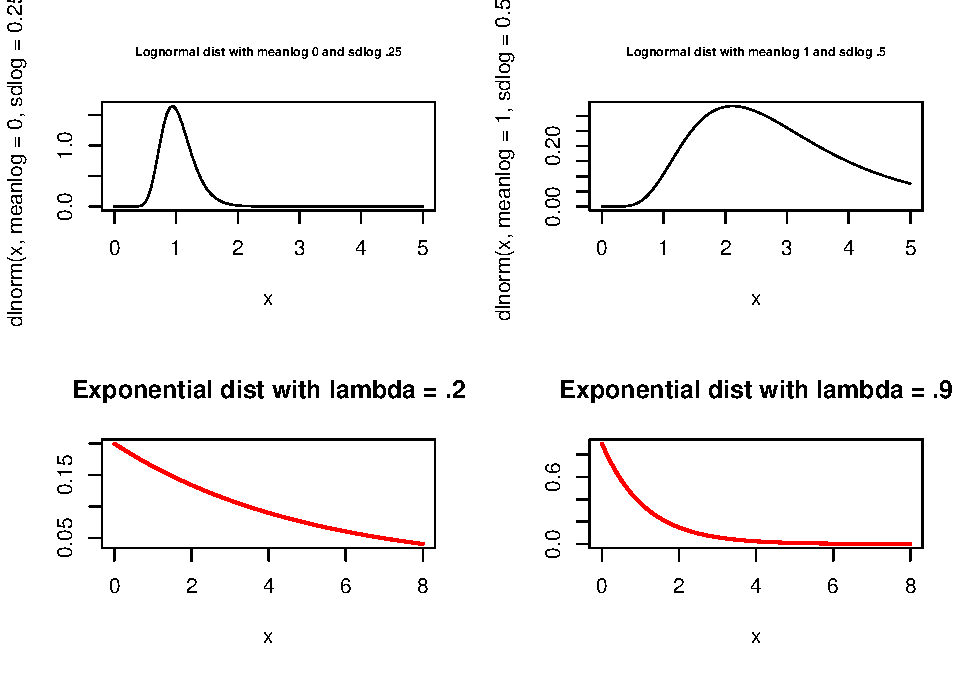
\includegraphics{Jessica-Yu_StatThesis_files/figure-latex/unnamed-chunk-1-1} \end{center}

\hypertarget{linear-mixed-effects-model}{%
\subsection{Linear mixed effects model}\label{linear-mixed-effects-model}}

In a linear mixed effects model, the amount of random effects that will be modeled depends on the research question at hand. Here, we will examine both a random intercepts model, where only the intercept of the model is assumed to have a random effects structure, as well as a random intercept and slope model, where in addition to intercept, the covariate time will also have a random effects structure. The random intercept model can be represented as: \[Y_{ij} = \beta_0 + \beta_1Trt_i + \beta_2Time_{ij} + b_{0j} + e_{ij},\] and the random slope model can be represented as: \[Y_{ij} = \beta_0 + \beta_1Trt_i + \beta_2Time_{ij} + b_{0j} + b_{1i}Time_{ij} + e_{ij}.\]

We use the \emph{lmerTest} package to fit the linear mixed effects model and evaluate random and fiexed effects. To evaluate significance of the treatment variable, we compare the performance and resulting p-values from 4 different Wald-type tests: KR, Satterthwaite, standard DF method, and \(t\)-as-\(z\). \(t\)-as-\(z\) and standard DF formula are not adjustments to account for smaller sample sizes, and are used as comparison to Satterthwaite and KR, since they are expected to be anti-conservative. Because the value of the treatment in our model is fixed at 0 in order to identify Type I error, we expect to see that the p-value to not be significant (\(p\) \textgreater{} .05) in an ideal scenario.

\hypertarget{evaluating-and-results}{%
\section{Evaluating and Results}\label{evaluating-and-results}}

After performing 400 replications of each condition at a significance level of .05, we evaluate robustness using Bradley's criterion, which considers a test to robust if the empirical error rate is between .025 and .075 Bradley (1978). In the following section, we will compare Type I error rates produced from KR and Satterthwaite methods as well as \(t\)-as-\(z\) and using the standard DF formula, further stratified by distribution and other manipulated parameters.
\begin{figure}

{\centering 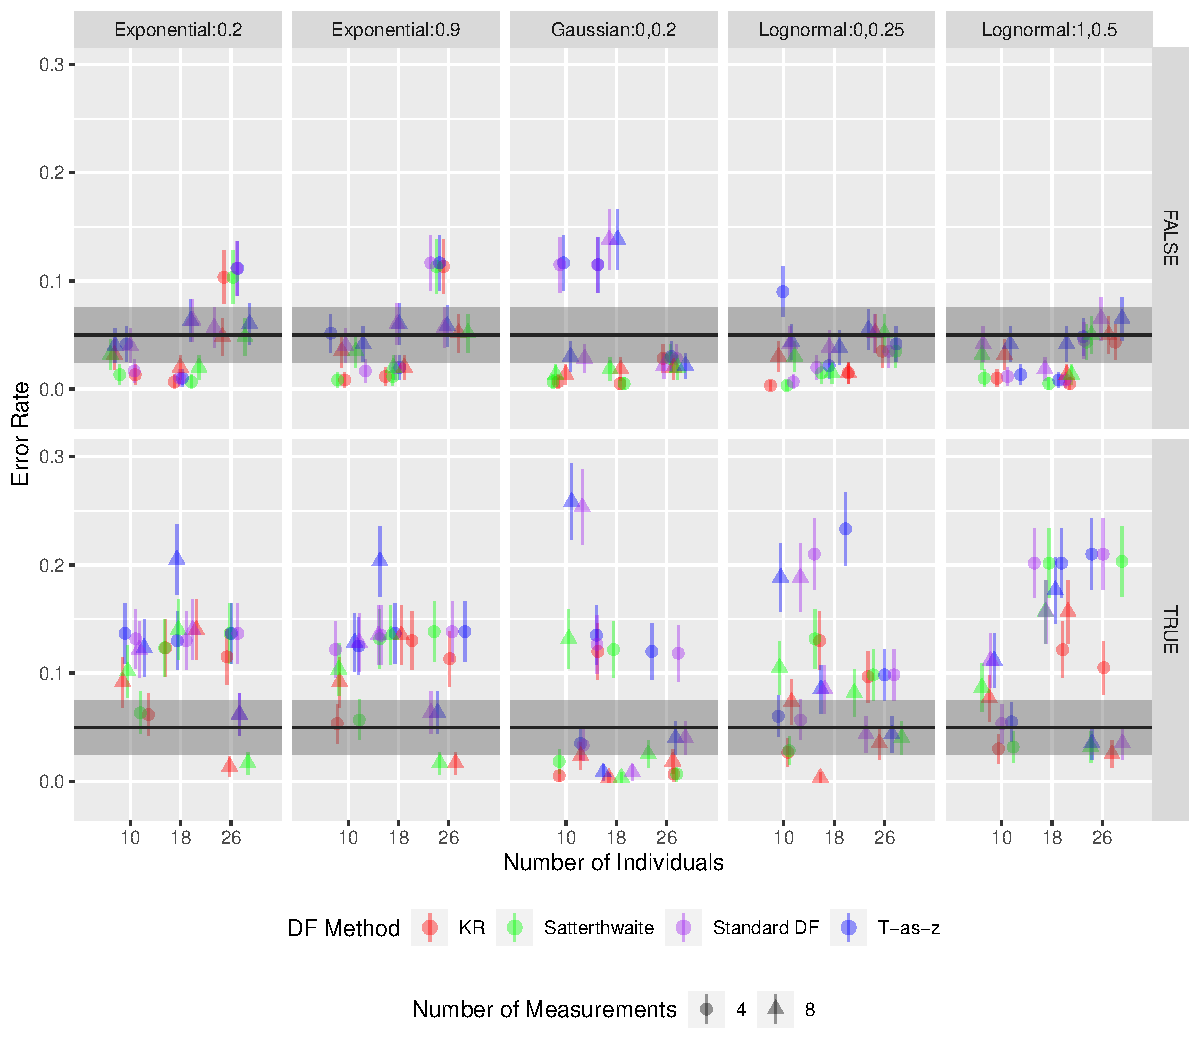
\includegraphics[angle=90]{Jessica-Yu_StatThesis_files/figure-latex/fig1-1} 

}

\caption{Type I Error Rates by DF method}\label{fig:fig1}
\end{figure}
Figure \ref{fig:fig1} displays error rates from all 4 degrees of freedom methods by distribution, parameters, complexity of random model, number of measurements, and number of samples. The shaded region indicates error rates that are considered robust by Bradley (1978)'s criterion. It is evident that there are varying patterns of performance by distribution. The common conception that larger sample sizes or large number of measurements can improve robustness is not necessarily evident across all distributions, for example in the case of the exponential distribution. One trend that appears to be evident across all three distributions is that when the degrees of freedom methods are applied to a random intercept model, a more structurally simple model, they yield more robust error rates in comparison to an application to the random slopes model.

In addition, when looking at performance of the 4 methods overall, we can see that the \(t\)-as-\(z\) and standard DF approach produce significantly more anti-conservative results, regardless of the values of other parameters. These trends align closely with a previous study by Luke (2017) examining only normal distributions.

In order to make more specific observations and identify trends, we will examine performance within each of the three distributions by sample size and number of measurements.

\hypertarget{exponential-distribution}{%
\subsection{Exponential Distribution}\label{exponential-distribution}}
\begin{figure}

{\centering 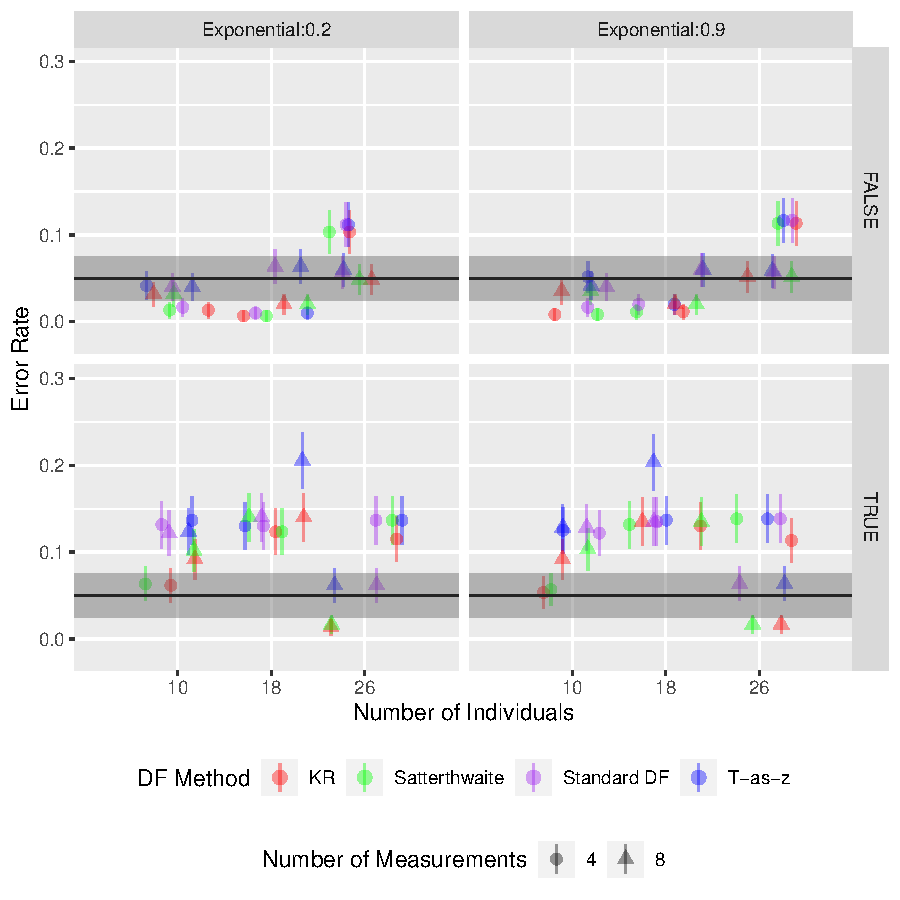
\includegraphics{Jessica-Yu_StatThesis_files/figure-latex/fig2-1} 

}

\caption{Type 1 Error Rates by DF method for Exponential Distribution}\label{fig:fig2}
\end{figure}
Our simulation results explore two exponential distributions, one with \(\lambda = .9\) and \(\lambda = .2\). Looking at figure \ref{fig:fig2}, at \(\lambda = .2\), we can see that in random slope models, comparing sample size of 10 to 26 marginally improves the DF methods, but only on those that are applied to conditions with more repeated measurements. The relationship between sample size and robustness is not linear, as increasing the sample size from 10 to 18 does not help DF methods achieve less anti-conservative error rates. On the other hand, in random intercept models, increasing the sample size did not improve the performance of DF methods, and in some cases were associated with more anti-conservative Type I error rates; in the case of sample size 26 and 4 measurements, Type I error rates performed significantly worse in comparison to smaller sample sizes, holding other conditions constant.

At \(\lambda = .9\), we see virtually the same trends in terms of the effect of sample size, complexity of model, and number of measurements on the performance of the DF methods. Overall, across both distributions, increasing the number of repeated measures impacted the DF methods' performance and increased robustness, while the effect of sample size was hard to pinpoint. Additionally, Kenward-Roger and Satterthwaite methods tended to produce more conservative error rates.

Despite having different parameter values, the application of DF methods to these two exponential distributions produce similar different trends in error rates. Considering that the two distributions have the same skewness and kurtosis values, we hypothesize whether this similarity in values contributes to the performance of the DF methods. Next, we will examine the performance of DF methods in lognormal distributions.

\hypertarget{lognormal}{%
\section{Lognormal}\label{lognormal}}
\begin{figure}

{\centering 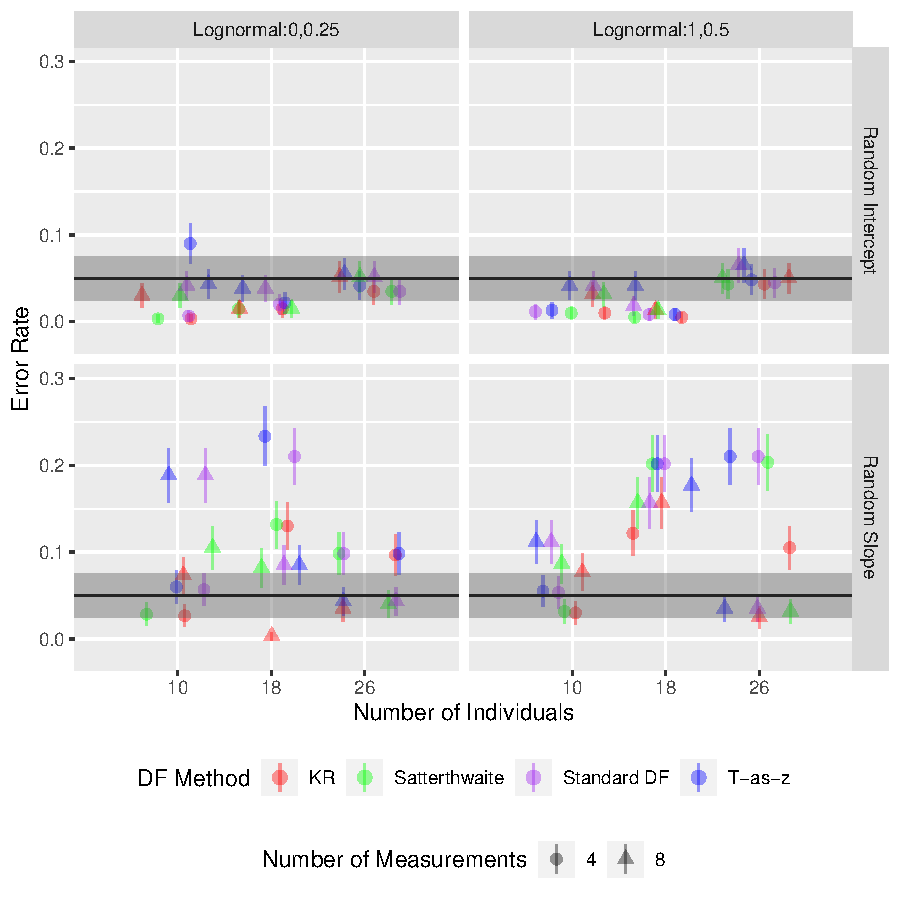
\includegraphics{Jessica-Yu_StatThesis_files/figure-latex/fig3-1} 

}

\caption{Type I Error Rates by DF Method for Lognormal Distribution}\label{fig:fig3}
\end{figure}
Figure \ref{fig:fig3} highlights Type I error rates produced by DF method for lognormal data. As seen in the exponential distribution, across the lognormal distributions, DF methods applied to random intercept models had consistently more robust error rates in comparison to random slope.

Our first lognormal distribution with parameters \((0,.25)\) has lower values of kurtosis and skewness. In the random slope model, increasing sample size from 10 to 18 only improves performance of the \(t\)-as-\(z\) and standard DF method when individuals have 8 measurements each, and in all other cases leads to less robustness. At sample size 26, DF methods are significantly more robust when applied to 8 measurements per individual rather than 4. In the random intercept model, we see a similar lack of consistent pattern of Type I error rates when sample size increases from 10 to 18, but at sample size 26 all methods regardless of number of measurements are robust.

On the other hand, with higher levels of skewness and kurtosis with a lognormal distribution with parameters \((1,.5)\), the effect of number of measurements and sample size are slightly different. Increasing the sample size from 10 to 18 has either no effect or an adverse effect on DF methods; in random intercept models the DF methods generally produce Type I error rates that are too conservative, and the opposite is seen in random slope models. Similar to the other lognormal distribution, DF methods applied to random intercept models of size 26 are all robust. The same difference between performance of DF methods of 4 and 8 measurements at size 26 in random slope models are observed, but that difference is widened. All DF methods at 4 measurements aside from the KR method have Type I error rates that almost 4 times the error rates at 8 measurements.

Based on comparisons between the two distributions, our results suggest that there are only slight differences that arise, suggesting that to a certain extent, distributions with greater skew and kurtosis may not significantly impact the performance of DF methods. In both distributions, DF methods applied to models with size 26 and 8 measurements were the most robust. Increasing sample size from 10 to 18 yields different Type I error rates across the two distributions, but it is difficult to discern a definite pattern.

\hypertarget{normal-distribution}{%
\section{Normal Distribution}\label{normal-distribution}}
\begin{figure}

{\centering 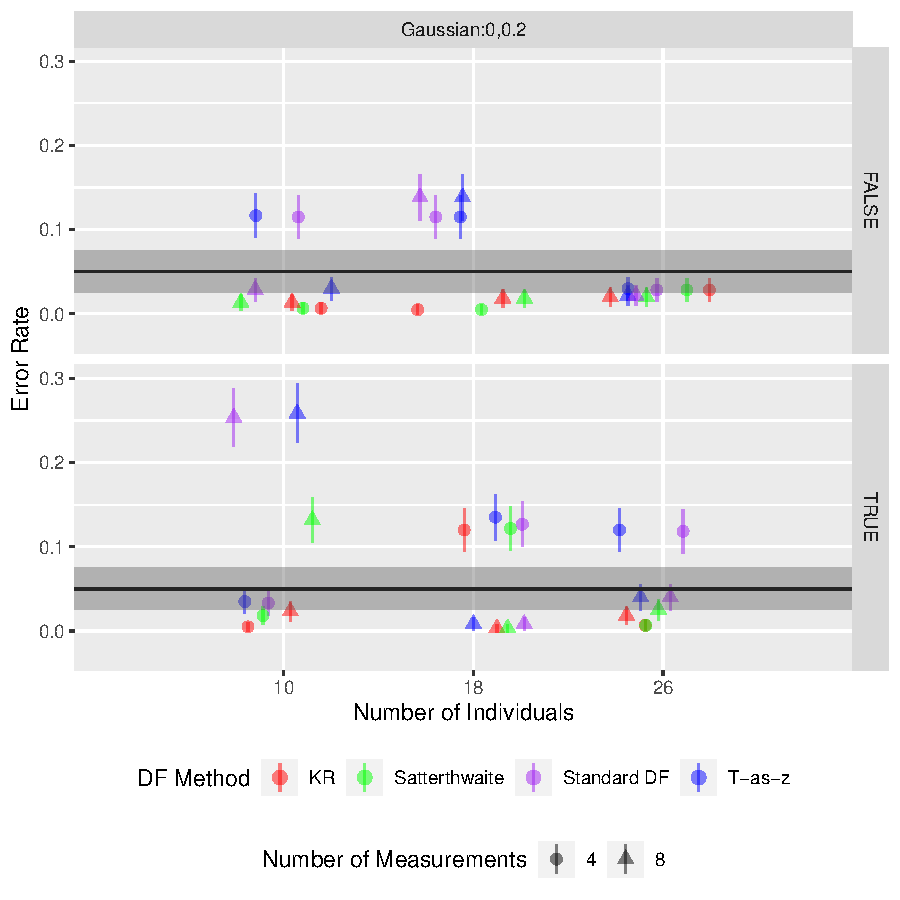
\includegraphics{Jessica-Yu_StatThesis_files/figure-latex/fig4-1} 

}

\caption{Type I Error Rates by DF Method for Normal Distribution}\label{fig:fig4}
\end{figure}
While nonnormal distributions are the focus of this study, comparing performance of DF methods to the normal distribution is important as a point of reference. As we can see in figure \ref{fig:fig4}, it is interesting to note how robustness has decreased for DF methods applied to the normal distribution compared to lognormal and exponential distributions, but it is also important to acknowledge that the methods, especially KR and Satterthwaite, produce conservative error rates, rather than anti-conservative ones. In most scenarios, KR and Satterthwaite remain unaffected when changing sample size. On the other hand, \(t\)-as-\(z\) and standard DF oftentimes produce the most anti-conservative error rates, but improvements arise when sample size is at 26.

Overall, in the normal distribution, there is a clearer distinction in performance of KR and Satterthwaite vs \(t\)-as-\(z\) and standard DF methods. Increasing the number of measurements is another factor that can affect Type I error rates produced by DF method within a particular method, rather than comparing across them.

\hypertarget{kr-vs-satterthwaite}{%
\subsection{KR vs Satterthwaite}\label{kr-vs-satterthwaite}}
\begin{figure}

{\centering 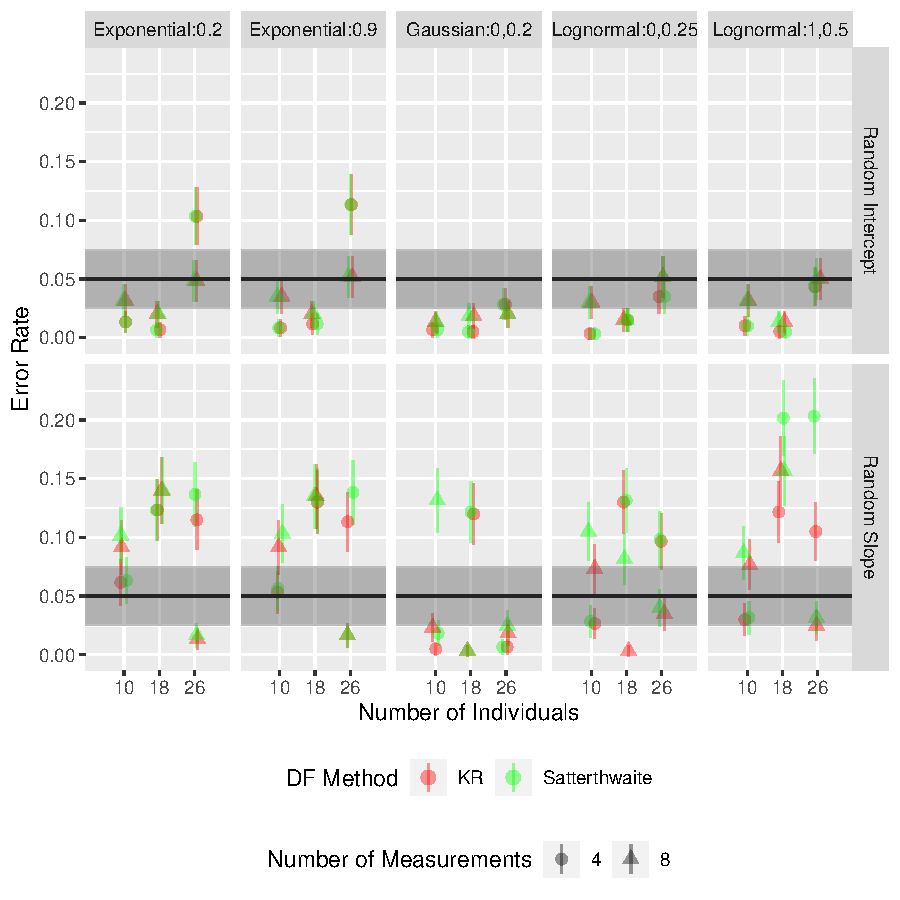
\includegraphics{Jessica-Yu_StatThesis_files/figure-latex/fig5-1} 

}

\caption{Type I Error Rates Produced by KR vs Satterthwaite}\label{fig:fig5}
\end{figure}
Comparing performance across all 4 methods has yielded significant evidence that KR and Satterthwaite are superior methods when using linear mixed models on small samples. Luke (2017) suggests that both KR and Satterthwaite are comparable solutions to obtain adequate Type I error. Figure \ref{fig:fig5} aims to narrow in on differences in performance between the two methods. One can see that across random intercept models, KR and Satterthwaite methods have identical performance. Looking more closely at random slope models, it appears that KR consistently produces more conservative error rates when holding distribution, sample size, and number of measurements constant. In two scenarios, of which models were of size 10 and 18, the KR method produced more conservative error rates, but were not robust, while the Satterthwaite method produced robust error rates.

While in a majority of cases KR is a viable solution when aiming to keep Type I error rates low, it is not necessarily the optimal DF choice in every scenario if the goal is to produce error rates closest to .05.

Tables for all error rates produced by 4 DF methods are located in the appendix \ref{table:tables}

\hypertarget{discussion}{%
\section{Discussion}\label{discussion}}

After comparing the error rates produced by DF methods across three distributions, three sample sizes, and two numbers of measurements and complexity of models totaling to 96 unique conditions, we find that overall, KR and Satterthwaite DF methods yield the most robust error rates when constructing LMM with small sample sizes. In addition, random slope models are significantly more complicated in terms of using DF methods to produce robust error rates, and also challenge the superiority of the KR method over the Satterthwaite method when looking at robustness of Type I errors of random slope models of smaller sample sizes.

This stark contrast in performance between random slope and random intercept models across all distributions requires further investigation. Barr, Levy, Scheepers, \& Tily (2013) suggest that LMM with maximal effects are preferable and can reduce Type I error rates, as random slope models can account for between individual variation in slopes and reduce residual variance. However, in their study the distribution of the variable of interest is normal, and random effects were generated from a bivariate normal distribution. In this simulation, random effects for the intercept and time were drawn from two nonnormal distributions which can further complicate the distribution of the outcome variable and complicate the fit of the model.

When comparing and constrasting performance of Satterthwaite and KR methods, which have both been demonstrated to be suitable options for producing robust Type I error, it seems that complexity of the model as well as sample size are two parameters that can differentiate their performance. In random intercept models, performance between the two methods are identical. In random slope models, KR is more conservative, and in a few conditions where the sample size is less than 26, it is too conservative in comparison to Satterthwaite. Given that KR is a further adjustment to Satterthwaite, its more conservative performance is not surprising; when constructing random slope LMM with smaller samples, \textasciitilde\textasciitilde it is important to consider both methods, as their performance may not be identical. \textasciitilde\textasciitilde{}

In terms of sample size and number of measurements, it appears that increasing the number of measurements increases the proportion of DF methods that produce robust Type I error rates in most conditions. Difference in DF method performance across measurement numbers is most evident in random slope models with samples of size 26. On the other hand, increasing sample size is not strongly associated with increased robustness of Type I error rates produced by DF methods. Increasing from sample size from 10 to 18 produces inconclusive patterns: sometimes DF methods produce even more anti-conservative error rates, and in other cases there is virtually no difference. In most cases, sample size of 26 is the most ideal for robustness, but in some nonnormal distributions robustness can only be achieved by also having more repeated measurements. It is plausible that the differences between a sample size of 10 and 18 are insignificant because both are too small in terms of a ``large-enough'' sample of size 30, so the DF methods are not impacted by this increase in sample. Models of sample size 26 may be ideal in some circumstances mainly because of its proximity to being considered sufficiently large enough.

While previous studies comparing DF methods focus primarily on normal distributions, the results from this study demonstrate that applying DF methods to LMM with nonnormal distributions and small sample sizes can still produce robust Type I error rates. However, careful consideration of the complexity of the model, number of measurements and individuals, as well as the skewness and kurtosis of the data must be considered, as they each have an effect on the DF method not only individually, but when interacting with other parameters as well. Overall, these results also indicate that Type I error rates are closest to .05 when employing Kenward-Roger and Satterthwaite methods.

\hypertarget{math-sci}{%
\chapter{Application}\label{math-sci}}

\hypertarget{application-to-longitudinal-study-about-childrens-health}{%
\section{Application to Longitudinal Study about Children's Health}\label{application-to-longitudinal-study-about-childrens-health}}

In this chapter, we will apply linear mixed models to a longitudinal study about children's health, and explore how inference of fixed effects can possibly change when using various degrees of freedom approximation methods.

\hypertarget{background}{%
\subsection{Background}\label{background}}

The National Longitudinal Study of Adolescent to Adult Health is a longitudinal study spanning 1994 to 2008 that surveyed a U.S sample of students in 7-12th grade in the 1994-95 school year (Harris \& Udry, 2022). Four waves of data were collected, in which the sample during the first wave was aged 13-18. Questions about mental health, socioeconomic status, and family background were collected, as well as physical measurements of height and weight.

One question of interest to consider is how salient life experiences that occur during adolescence, such as being exposed to alcohol or being in a physical altercation, may impact changes to one's physical health over time. One way to capture physical health is through BMI, which is shown to follow a skewed nonnormal distribution (Penman \& Johnson, 2006). With this in mind, we can employ methods of degrees of freedom adjustment. While this dataset is large and encompasses approximately 5,000 students, the scope of this application will be narrowed in order to examine the performance of degrees of freedom methods, which are sensitive to sample size.

We will be focusing on Chinese female respondents who completed at least three waves of the study, which amounts to a sample size of 12. After initial exploration, alcohol use was chosen for the model. It is hypothesized that early exposure to substances could potentially affect changes in weight.

The following variables were assessed in the first wave of the study (1994):
- Alcohol: has the child ever had alcohol? (Yes/No)
- Age

\hypertarget{exploration}{%
\subsection{Exploration}\label{exploration}}
\begin{center}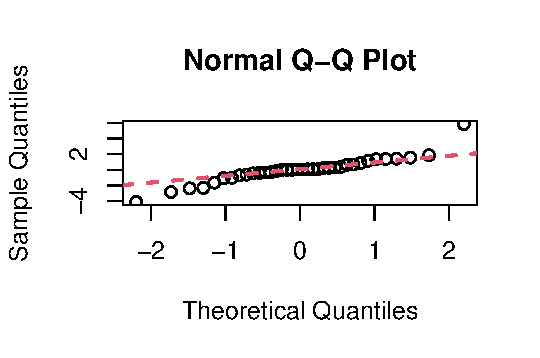
\includegraphics{Jessica-Yu_StatThesis_files/figure-latex/unnamed-chunk-5-1} \end{center}

From this histogram depicting distribution of BMI, we can see that it follows a nonnormal trend. The skewness is .95 and the kurtosis is 3.39.
\begin{figure}

{\centering 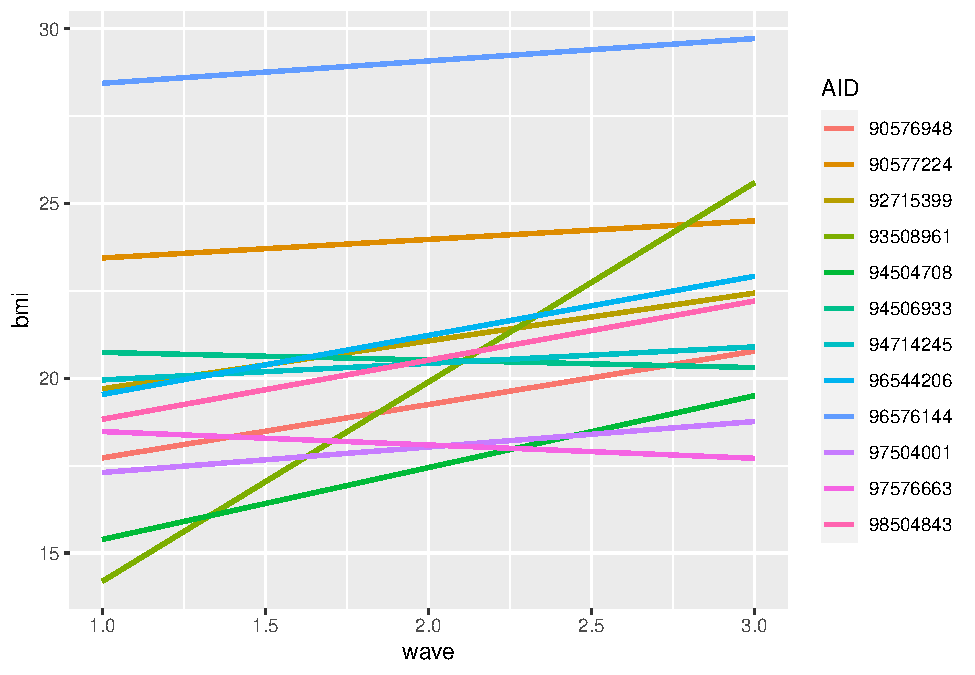
\includegraphics{Jessica-Yu_StatThesis_files/figure-latex/intercept-1} 

}

\caption{Changes in BMI by Individual}\label{fig:intercept}
\end{figure}
Figure \ref{fig:intercept} depicts changes in BMI over time for each individual in the study. The wide variation in BMI values between individuals suggest that including random effects for the intercept would be beneficial. Additionally, different rates of change in BMI across the 3 waves between individuals would suggest that an additional random effect for time is worth exploring.
\begin{figure}

{\centering 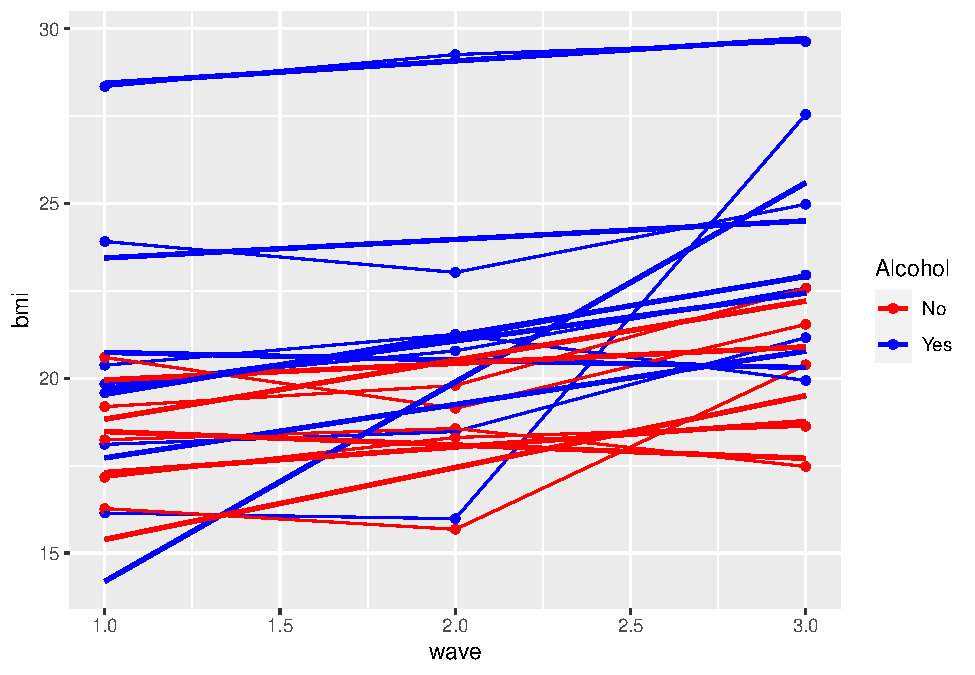
\includegraphics{Jessica-Yu_StatThesis_files/figure-latex/alcohol-1} 

}

\caption{Changes in BMI by Individual and Alcohol Use}\label{fig:alcohol}
\end{figure}
In a longitudinal study examining youth substance use and body composition, Pasch, Velazquez, Cance, Moe, \& Lytle (2012) found that baseline alcohol use is associated with lower values of BMI at follow-up. The opposite pattern can be seen in Figure \ref{fig:alcohol}. Individuals who had consumed alcohol during the first wave had higher BMI values across all time points. While the data may not be consistent with other research, it highlights the importance of substance use as a potential predictor of BMI.

While our sample size is small, our initial exploration of alcohol use suggests that it may be salient predictor for BMI. In addition, there are unique patterns of BMI change over time by individual, which suggests that creating a mixed effects model with random effects for time and intercept may be useful.

\hypertarget{linear-mixed-model}{%
\subsection{Linear Mixed Model}\label{linear-mixed-model}}

Because we have repeated measurements of the same individual in this study, a regular linear model would not be appropriate as it assumes independence; implementing this model would inflate Type I error rates.
\begin{table}

\caption{(\#tab:lm, cap)Linear Model Output}
\centering
\begin{tabular}[t]{l|r|r|r|r}
\hline
term & estimate & std.error & statistic & p.value\\
\hline
(Intercept) & 9.71 & 4.736 & 2.05 & 0.049\\
\hline
alcohol1 & 3.13 & 1.044 & 3.00 & 0.005\\
\hline
age\_at\_start & 0.42 & 0.288 & 1.46 & 0.154\\
\hline
wave & 1.32 & 0.629 & 2.10 & 0.044\\
\hline
\end{tabular}
\end{table}
Table \ref{tab:lm} shows the results of implementing a linear model with alcohol, age at first wave, and time as predictors. Alcohol use and time are significant predictors in this model. This will only used as a comparison to the other linear mixed models.

\hypertarget{intercept-only-model}{%
\subsection{Intercept only model}\label{intercept-only-model}}

We would hypothesize that changes in weight may vary less within a person, as opposed to comparing changes in weight across two separate individuals. Thus, we fit an intercept only model, allowing the intercept to vary by individual. Alcohol, age at first wave, and time are the fixed effects.

\textbackslash begin\{table\}

\textbackslash caption\{(\#tab:intercept\_KR)Fixed Effects for Random Intercept Model Using KR\}
\centering
\begin{tabular}[t]{l|r|r|r|r|r}
\hline
term & estimate & std.error & statistic & df & p.value\\
\hline
(Intercept) & 9.71 & 7.274 & 1.335 & 9.22 & 0.214\\
\hline
alcohol1 & 3.13 & 1.653 & 1.897 & 9.00 & 0.090\\
\hline
age\_at\_start & 0.42 & 0.456 & 0.921 & 9.00 & 0.381\\
\hline
wave & 1.32 & 0.403 & 3.272 & 23.00 & 0.003\\
\hline
\end{tabular}
\textbackslash end\{table\}
\begin{table}
\centering
\begin{tabular}[t]{l|l|r}
\hline
group & term & estimate\\
\hline
AID & sd\_\_(Intercept) & 2.57\\
\hline
Residual & sd\_\_Observation & 1.97\\
\hline
\end{tabular}
\end{table}
First, we can examine the output of the fixed effects similar to how a regular linear regression model is interpreted. Table @ref(tab:intercept\_KR) shoes that time is the only significant effect. This means that conditional on the random effects, each wave increases the predicted BMI by 1.32. Next, we turn to the random effects output in table @ref(tab:intercept\_rand). The variance for individuals (represented by \texttt{AID}), which depicts variability across individuals, is 6.626, while the residual variance, representing within-subject variability is 3.895. The significantly larger variance across individuals compared to within individuals suggests that this model is more optimal than a regular linear regression model since differences in variability are apparent. The interclass correlation is .63, which indicates that weight measurements taken of the same individual have slightly higher similarity than those of different individuals.
\begin{center}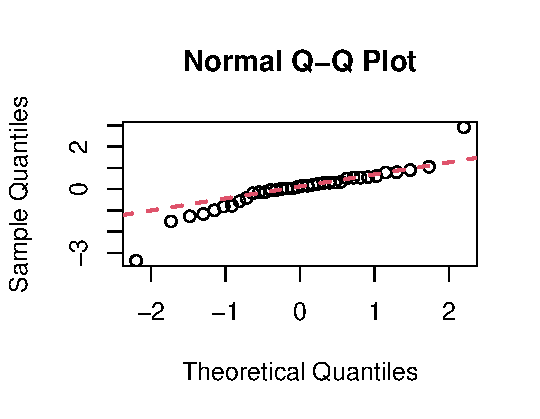
\includegraphics{Jessica-Yu_StatThesis_files/figure-latex/unnamed-chunk-6-1} \end{center}
\begin{center}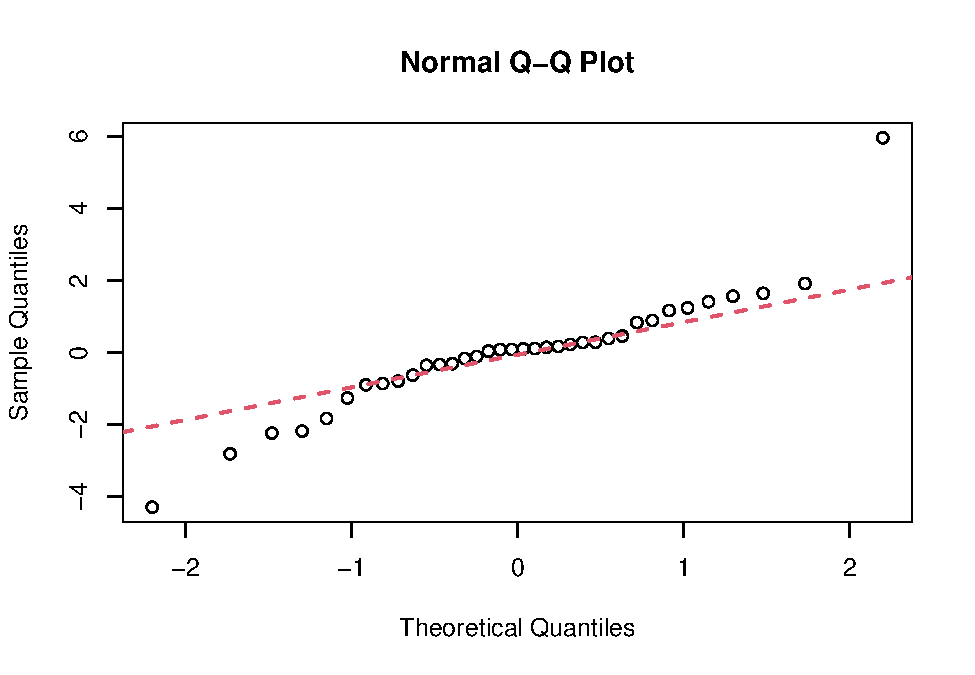
\includegraphics{Jessica-Yu_StatThesis_files/figure-latex/unnamed-chunk-6-2} \end{center}

The residuals vs fitted plot indicates no heterogeneity in the residuals, and the qqplot indicates that for the most part residuals are normally distributed. The assumptions for fitting a random slope linear mixed model are met.

\textbackslash begin\{table\}

\textbackslash caption\{(\#tab:compare\_intercept)Comparison of Fixed Effects P-Values in Random Intercept Model\}
\centering
\begin{tabular}[t]{l|l|l}
\hline
term & Satterthwaite\_p.value & KR\_p.value\\
\hline
(Intercept) & 0.214028860057237 & 0.214028858602635\\
\hline
alcohol1 & 0.0903585620561796 & 0.0903585607408565\\
\hline
age\_at\_start & 0.380940524102144 & 0.380940522986174\\
\hline
wave & 0.00335031625142439 & 0.00335031627116489\\
\hline
\end{tabular}
\textbackslash end\{table\}

The summary output referenced above uses Kenward-Roger DF approximation. Table @ref(tab:compare\_intercept) compares the summary output comparing Satterthwaite and Kenward-Roger. There is no significant difference between performance of the two DF methods, which aligns with results of our random intercept models from our simulation study

\hypertarget{intercept-and-random-slope}{%
\subsection{Intercept and random slope}\label{intercept-and-random-slope}}

\textbackslash begin\{table\}

\textbackslash caption\{(\#tab:slope\_kr)Fixed Effects for Random Slope Model Using KR\}
\centering
\begin{tabular}[t]{l|r|r|r|r|r}
\hline
term & estimate & std.error & statistic & df & p.value\\
\hline
(Intercept) & 11.644 & 2.881 & 4.041 & 25.71 & 0.000\\
\hline
alcohol1 & 3.461 & 1.666 & 2.077 & 9.64 & 0.066\\
\hline
real\_age & 0.394 & 0.209 & 1.885 & 16.52 & 0.077\\
\hline
wave & -0.060 & 0.862 & -0.069 & 26.70 & 0.945\\
\hline
\end{tabular}
\textbackslash end\{table\}

In this model, we add a random effect of time as well as random intercept. This means that we are assuming that for each individual, the relationship between time and BMI is unique. There are no significant effects when using the KR method. Variability in BMI across individuals is 16.388, and the residual variance is 2.352. The variance for time is 1.324, which represents variability across individual's BMI rates of change. We see that imposing variability between each individual's relationship of time vs BMI reduces some of the residual variance. When we accounted for some of the variation through each individual's weight changes over time, time as a predictor was no longer signficant as it was in the random intercepts only model.

Conditions for the model are met as seen by the figures below.
\begin{center}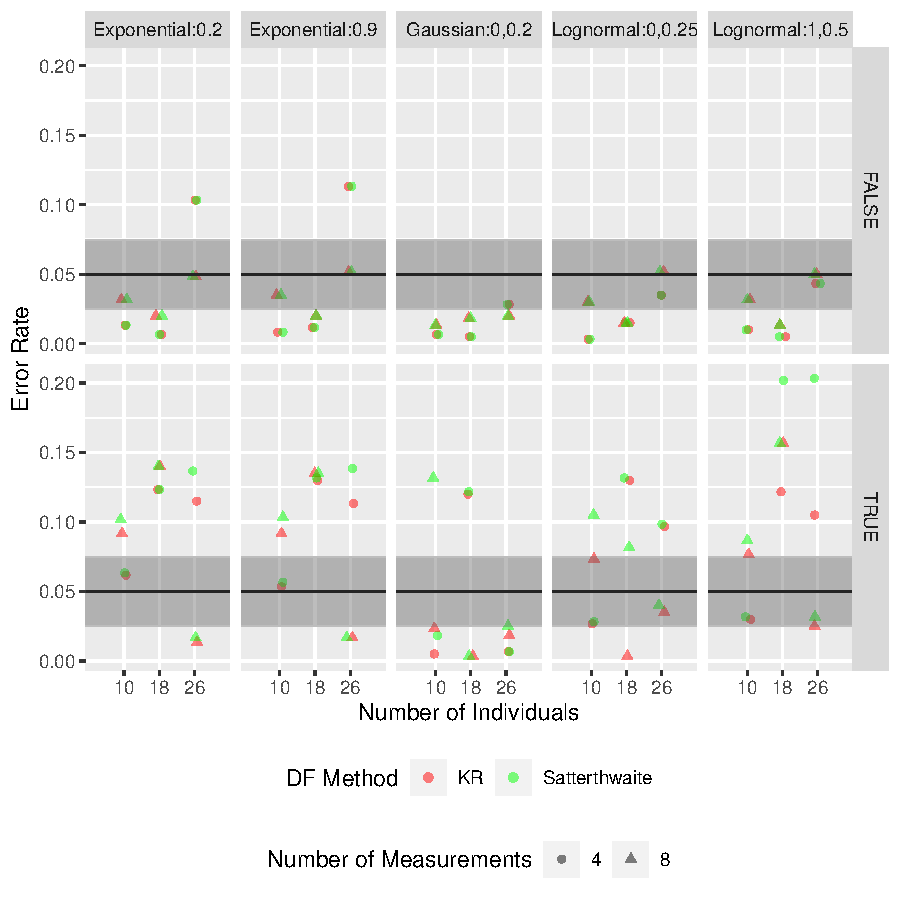
\includegraphics{Jessica-Yu_StatThesis_files/figure-latex/unnamed-chunk-7-1} \end{center}
\begin{center}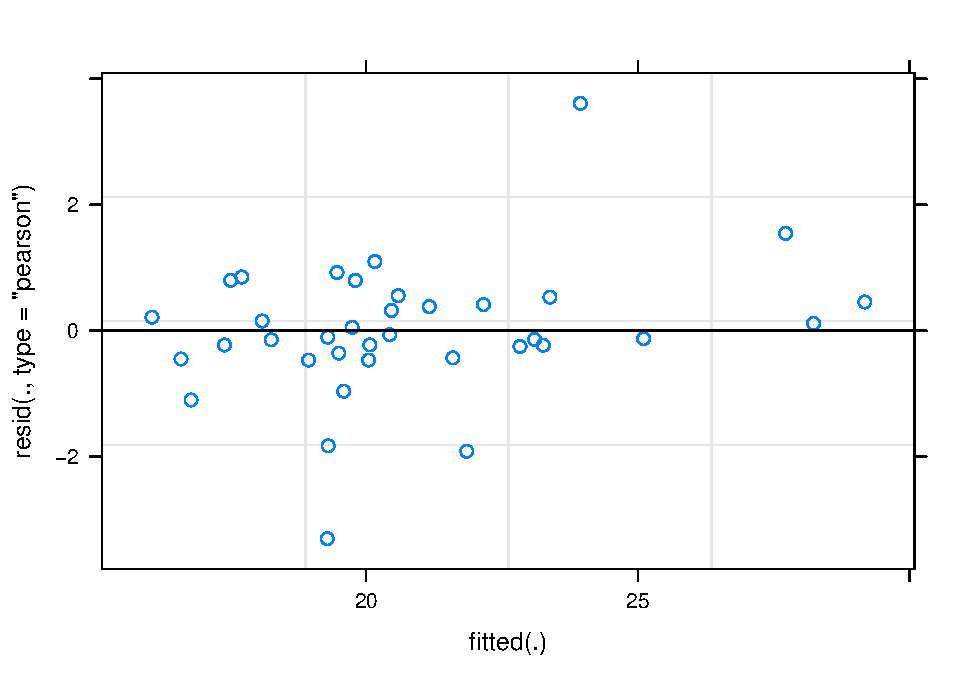
\includegraphics{Jessica-Yu_StatThesis_files/figure-latex/unnamed-chunk-7-2} \end{center}

\textbackslash begin\{table\}

\textbackslash caption\{(\#tab:compare\_slope)Comparison of Fixed Effects P-Values in Random Slope Model\}
\centering
\begin{tabular}[t]{l|l|l}
\hline
term & Satterthwaite\_p.value & KR\_p.value\\
\hline
(Intercept) & 0.000213283766249562 & 0.000426895805163504\\
\hline
alcohol1 & 0.0459153731793183 & 0.0655425035327326\\
\hline
real\_age & 0.0572004159149207 & 0.0771903662035183\\
\hline
wave & 0.942264459160284 & 0.945433676863754\\
\hline
\end{tabular}
\textbackslash end\{table\}

Earlier evaluation of fixed effects uses KR DF method, but @ref(tab:compare\_slope) shows that significance of fixed effects differ when using Satterthwaite versus KR. In the random slope model, alcohol not a significant effect when using KR, but is significant when using Satterthwaite. This difference affects our interpretation of the model and conclusions that are drawn.

\hypertarget{discussion-1}{%
\section{Discussion}\label{discussion-1}}

We have demonstrated implementing two linear mixed models on a data set that is small and with a nonnormal continuous outcome. Imposing random effects structure to isolate variation between individuals apart from overall variation improved the model and reduced the number of predictors that were significant. One key result was that comparing KR and Sattherthwaite DF methods resulting in varying significant predictors in the random slope model. One additional predictor, alcohol, was a significant fixed effect when using Satterthwaite, the default output summary for \emph{lmerTest}, in comparison to KR. Which method is preferable?

Looking at the results from our simulation study, we can identify which condition most closely resembles the children data, and determine if KR or Satterthwaite would produce more robust results. There was no difference in the fixed effects of the random intercept model, so we only focus on the random slopes model. The skewness and kurtosis values for the application data align most closely with that of the lognormal distribution \(X\sim\mathit{Log}(0,.25).\) We will look at the performance of the two DF methods in this distribution, in a random slope model with a sample size of 10 and 4 measurements per individual. In reference to Figure \ref{fig:fig5}, we see that the performance of KR and Satterthwaite are virtually the same. If this is the case, our preference will still be towards KR as it tends to produce slightly less anti-conservative Type I error rates.

Ultimately, our application study supports the idea that linear mixed models can be applied to small samples when using KR or Satterthwaite DF methods. While performance between the two can be equally robust in theory, they can possibly lead to different significant fixed effects and conclusions about data overall.

\hypertarget{conclusion-1}{%
\chapter*{Conclusion}\label{conclusion-1}}
\addcontentsline{toc}{chapter}{Conclusion}

In this study, we explored how Type I error rates from 4 different DF methods: Kenward-Roger, Satterthwaite, standard DF method, and \(t\)-as-\(z\) compare when evaluating significance of fixed effects of linear mixed models, particularly in small samples and in nonnormal distributions. Using a range of sample sizes, number of measurements, lognormal, and exponential distributions, as well as both random intercept and random slope models, we found distinct differences in performance of DF methods. DF methods applied to random slope models produced more anti-conservative Type I error rates in comparison to random intercept models. While increasing the number of measurements appears to increase robustness of most methods, the same effect for sample size was not identified. Across the 4 DF methods, KR and Satterthwaite DF were consistently more robust and less anti-conservative; while both are preferable, KR is consistently less anti-conservative, which makes it a more optimal choice. When fitting linear mixed models to a subset of a children's longitudinal health survey, we find that the significance of fixed effects differs between KR and Satterthwaite DF. Our results indicate that performance of DF methods can vary greatly in small sample sizes, which can in turn impact the conclusions drawn about the fixed effects. Further exploration into other nonnormal distributions and other criteria that could impact DF method is needed.

\appendix

\hypertarget{the-first-appendix}{%
\chapter{The First Appendix}\label{the-first-appendix}}

This first appendix includes all of the R chunks of code that were hidden throughout the document (using the \texttt{include\ =\ FALSE} chunk tag) to help with readibility and/or setup.

\hypertarget{in-the-main-file-refref-labels}{%
\section{In the main file \ref{ref-labels}:}\label{in-the-main-file-refref-labels}}

\hypertarget{in-chapter-refref-labels}{%
\section{In Chapter \ref{ref-labels}:}\label{in-chapter-refref-labels}}

\hypertarget{the-second-appendix}{%
\chapter{The Second Appendix}\label{the-second-appendix}}

\hypertarget{corrections}{%
\chapter*{Corrections}\label{corrections}}
\addcontentsline{toc}{chapter}{Corrections}

A list of corrections after submission to department.

Corrections may be made to the body of the thesis, but every such correction will be acknowledged in a list under the heading ``Corrections,'' along with the statement ``When originally submitted, this honors thesis contained some errors which have been corrected in the current version. Here is a list of the errors that were corrected.'' This list will be given on a sheet or sheets to be appended to the thesis. Corrections to spelling, grammar, or typography may be acknowledged by a general statement such as ``30 spellings were corrected in various places in the thesis, and the notation for definite integral was changed in approximately 10 places.'' However, any correction that affects the meaning of a sentence or paragraph should be described in careful detail. The files samplethesis.tex and samplethesis.pdf show what the ``Corrections'' section should look like. Questions about what should appear in the ``Corrections'' should be directed to the Chair.

\backmatter

\hypertarget{references}{%
\chapter*{References}\label{references}}
\addcontentsline{toc}{chapter}{References}

\noindent

\setlength{\parindent}{-0.20in}
\setlength{\leftskip}{0.20in}
\setlength{\parskip}{8pt}

\hypertarget{refs}{}
\leavevmode\hypertarget{ref-barr_random_2013}{}%
Barr, D. J., Levy, R., Scheepers, C., \& Tily, H. J. (2013). Random effects structure for confirmatory hypothesis testing: Keep it maximal. \emph{Journal of Memory and Language}, \emph{68}(3), 255--278. \url{http://doi.org/10.1016/j.jml.2012.11.001}

\leavevmode\hypertarget{ref-bradley}{}%
Bradley, J. V. (1978). Robustness? \emph{British Journal of Mathematical and Statistical Psychology}, \emph{31}(2), 144--152. \url{http://doi.org/https://doi.org/10.1111/j.2044-8317.1978.tb00581.x}

\leavevmode\hypertarget{ref-Simtest}{}%
Fialkowski, A. C. (2018). \emph{SimMultiCorrData: Simulation of correlated data with multiple variable types}. Retrieved from \url{https://CRAN.R-project.org/package=SimMultiCorrData}

\leavevmode\hypertarget{ref-fitzmaurice_applied_2011}{}%
Fitzmaurice, G. M., Laird, N. M., \& Ware, J. H. (2011). \emph{Applied longitudinal analysis} (2nd ed). Hoboken, N.J: Wiley.

\leavevmode\hypertarget{ref-harris_national_2022}{}%
Harris, K. M., \& Udry, J. R. (2022). National longitudinal study of adolescent to adult health (add health), 1994-2018 {[}public use{]}. Carolina Population Center, University of North Carolina-Chapel Hill {[}distributor{]}, Inter-university Consortium for Political; Social Research {[}distributor{]}. \url{http://doi.org/10.3886/ICPSR21600.v24}

\leavevmode\hypertarget{ref-luke_evaluating_2017}{}%
Luke, S. G. (2017). Evaluating significance in linear mixed-effects models in r. \emph{Behavior Research Methods}, \emph{49}(4), 1494--1502. \url{http://doi.org/10.3758/s13428-016-0809-y}

\leavevmode\hypertarget{ref-pasch_youth_2012}{}%
Pasch, K. E., Velazquez, C. E., Cance, J. D., Moe, S. G., \& Lytle, L. A. (2012). Youth substance use and body composition: Does risk in one area predict risk in the other? \emph{Journal of Youth and Adolescence}, \emph{41}(1), 14--26. \url{http://doi.org/10.1007/s10964-011-9706-y}

\leavevmode\hypertarget{ref-penman_changing_2006}{}%
Penman, A. D., \& Johnson, W. D. (2006). The changing shape of the body mass index distribution curve in the population: Implications for public health policy to reduce the prevalence of adult obesity. \emph{Preventing Chronic Disease}, \emph{3}(3), A74--A74. Retrieved from \url{https://pubmed.ncbi.nlm.nih.gov/16776875}

\leavevmode\hypertarget{ref-zeng_chinese_2017}{}%
Zeng, Y., Vaupel, J., Xiao, Z., Liu, Y., \& Zhang, C. (2017). Chinese longitudinal healthy longevity survey (CLHLS), 1998-2014. Inter-university Consortium for Political; Social Research {[}distributor{]}. \url{http://doi.org/10.3886/ICPSR36692.v1}

% Index?

\end{document}
